\documentclass{IEEEtran}
\usepackage{csquotes}
\usepackage{url}
\usepackage{graphicx}
\usepackage{caption}
\usepackage{xcolor,colortbl}
\usepackage{textcomp} 
\usepackage{listings}
\usepackage{enumitem}
\usepackage{float}
\usepackage{subfig}

\newcommand{\mc}[2]{\multicolumn{#1}{c}{#2}}
\definecolor{Gray}{gray}{0.95}
\definecolor{LightCyan}{rgb}{0.88,1,1}

\newcolumntype{a}{>{\columncolor{Gray}}l}
\newcolumntype{b}{>{\columncolor{white}}c}

\graphicspath{{./img/}}


% Listings

\lstset{numbers=none,numberblanklines=false,columns=fullflexible,basicstyle=\ttfamily,linewidth=\columnwidth,breaklines=true}

\newcommand{\CodeSymbol}[1]{\bfseries\textcolor{violet}{#1}}   % Code associated to defining styles
\newcommand{\InitColor}[1]{\bfseries\textcolor{orange}{#1}}   % Code associated to defining styles
\newcommand{\RedColor}[1]{\bfseries\textcolor{red}{#1}}   % Code associated to defining styles
\newcommand{\PairColor}[1]{\bfseries\textcolor{blue}{#1}}   % Code associated to defining styles
\newcommand{\CustomFunction}[1]{\bfseries\textcolor{magenta}{#1}}   % Code associated to defining styles

\definecolor{codegray}{gray}{0.95}
\definecolor{commentgray}{gray}{0.35}

\makeatletter

\lstdefinelanguage{clingo}{%
  basicstyle=\footnotesize\ttfamily,%
  backgroundcolor=\color{codegray},%
  showstringspaces=false,%
  alsoletter=0123456789,%
  columns=fullflexible,%
  resetmargins=true,%
  breaklines=true,%
  keywords=[3]{&,&dom,&sum,&diff,&show},%
  morecomment=[l]{\#\ },%
  morecomment=[l]{\%\ },%
  morestring=[b]",%
  stringstyle={\itshape},%
  commentstyle={\color{commentgray}},%
  literate={init}{{\InitColor{init}}}1
           {not}{{\RedColor{not }}}1
           {pair}{{\PairColor{pair}}}1
           {onNode}{{\CustomFunction{onNode}}}1
           {occurs}{{\CustomFunction{occurs}}}1
           {action}{{\CustomFunction{action}}}1
           {move}{{\CodeSymbol{move}}}1
           {robot}{{\CodeSymbol{robot}}}1
           {robotMove}{{\CustomFunction{robotMove}}}1
           {onRobot}{{\CustomFunction{onRobot}}}1
           {deliver}{{\CustomFunction{deliver}}}1
           {onShelf}{{\CustomFunction{onShelf}}}1
           {order}{{\CustomFunction{order}}}1
           {goal}{{\CustomFunction{goal}}}1
           {pickingStation}{{\CustomFunction{pickingStation}}}1
           {nodeAt}{{\CodeSymbol{nodeAt}}}1
           {object}{{\CodeSymbol{object}}}1
           {value}{{\CodeSymbol{value}}}1
           {\#const}{{\CodeSymbol{\#const }}}1
           {\#show}{{\CodeSymbol{\#show }}}1
           {\#minimize}{{\CodeSymbol{\#minimize }}}1
           {\#base}{{\CodeSymbol{\#base }}}1
           {\#theory}{{\CodeSymbol{\#theory }}}1
           {\#count}{{\CodeSymbol{\#count }}}1
           {\#external}{{\CodeSymbol{\#external }}}1
           {\#program}{{\CodeSymbol{\#program }}}1
           {\#script}{{\CodeSymbol{\#script }}}1
           {\#end}{{\CodeSymbol{\#end }}}1
           {\#heuristic}{{\CodeSymbol{\#heuristic }}}1
           {\#edge}{{\CodeSymbol{\#edge }}}1
           {\#project}{{\CodeSymbol{\#project }}}1
           {\#show}{{\CodeSymbol{\#show }}}1
           {\#sum}{{\CodeSymbol{\#sum }}}1%
}

\newcommand\opstyle{\CodeSymbol} % <--- customise operator style here

% Hook into listings
\lst@AddToHook{OutputOther}{\ProcessOther@silmeth}

% helper macro
\newcommand\ProcessOther@silmeth
{%
  \ifnum\lst@mode=\lst@Pmode%     % If we're in `Processing' mode...
    \def\lst@thestyle{\opstyle}%  % ... redefine the style locally
  \fi%
}

\makeatother

\newcommand{\Sim}{{\raise.17ex\hbox{\ensuremath{\scriptstyle\sim}}}}

\begin{document}

\title{CSE 579: Knowledge Representation and Reasoning}
\author{Claudio Rodriguez Rodriguez}
\maketitle

\section{Introduction}

The goal of the project is to apply Knowledge Representation and Reasoning teachings of Answer Set Programming. We use clingo, a tool developed by the Potsdam Answer Set Solving Collection (Potassco), to implement the Concepts. Using clingo, we can show the expressive power of ASP and how it allows solving a combinatorial problem with relative ease. With ASP, we can focus on the problem domain to deliver a solution while abstracting how to implement it.

We also observe that a single rule in the problem's solution creates "collaboration" between the robots. We also confirm that clingo takes less than a second for all the given input instances. We present a table with the results for all the sample instances provided in the ASP Challenge 2019\cite{cse579:AutomatedWarehouseScenario}. 

Our project focused on respecting the Constraints of the problem and reaching the expected number of steps. But to showcase our results, we created visualizations using the same tool used to validate the results while developing the solution, Asprilo. 

\begin{quotation}
  $asprilo$ is a benchmarking framework to study typical scenarios in intra-logistics and warehouse automation with multiple mobile robots. 
  Asprilo contains multiple tools, but the one that we used during the project is the Visualizer.\cite{cse579:asprilo}
\end{quotation}
 
To validate our answers, we use the Visualizer tool as part of the Asprilo Benchmarking framework. We only showcase one problem to present the collaboration of the robots.

\section{Description of Solution}

During the class, Dr. Lee mentioned a methodology of Answer Set Programming\cite{cse579:Methodology}, and it is defined as follows:

\begin{enumerate}
  \item \textbf{Generate}: Create a Search space of potential solutions.
  \item \textbf{Define}: Define new variables from other variables to simplify some processes.
  \item \textbf{Test}: Remove elements on the search space that are not part of the solution.
\end{enumerate}

Afterward, we create our goal state in mind and start adding constraints to the solution space. We studied the following high-level structure to tackle crafting a solution:

\begin{enumerate}
  \item Sort and object declarations. We translate the input from the ASP Challenge 2019 problems into more useful objects, such as the one observer in Listing~\ref{code:SnippetSortDeclaration}.
  \lstinputlisting[
    label={code:SnippetSortDeclaration}, caption={State $goal$ definition}, language=clingo,
    linewidth=3.2in,
    firstline=24, lastline=28
  ]{./src/main.lp}
  \item State constraints (\textit{actions}). Robots can perform multiple actions, and we show the most relevant in Listing~\ref{code:SnippetActionDeclaration}.
  \lstinputlisting[
    label={code:SnippetActionDeclaration}, caption={Effect of deliver action}, language=clingo,
    linewidth=3.2in,
    firstline=41, lastline=46
  ]{./src/main.lp}
  \item Effect and preconditions of actions. All actions have an effect on the state, and they must be carefully worded such as in Listing~\ref{code:SnippetEffectDelivering}.
  \lstinputlisting[
    label={code:SnippetEffectDelivering}, caption={Effect of Delivering an Order}, language=clingo,
    linewidth=3.2in,
    firstline=166, lastline=175
  ]{./src/main.lp}
  \item Action constraints. Part of the $Test$ Method in our Methodology of ASP, and the Listing~\ref{code:SnippetConstraintShelf} shows a critical constraint to allow collaboration.
  \lstinputlisting[
    label={code:SnippetConstraintShelf}, caption={Robot can't pass through shelf if it has a shelf}, language=clingo,
    linewidth=3.2in,
    firstline=84, lastline=92
  ]{./src/main.lp}
  \item Domain independent axioms. These constraints help code the law of inertia, which means an object will remain on the same place in the next timestamp if there was no action on it (Listing~\ref{code:LawInertia}).
  \lstinputlisting[
    label={code:LawInertia}, caption={Law of inertia for product on a shelf}, language=clingo,
    linewidth=3.2in,
    firstline=200, lastline=203
  ]{./src/main.lp}
\end{enumerate}

Asprilo defines the same input as the description of the Automated Warehouse Problem\cite{cse579:AutomatedWarehouseScenario}. We replace the output from the original problem with the definition expected by Asprilo. This simple change allowed for increased iterability speed. 

\lstinputlisting[
    label={Snippet of output}, caption={Snippet of Output used by Asprilo}, language=clingo,
    linewidth=3.2in,
    firstline=49, lastline=49
  ]{./src/main.lp}

Hoos and Stützle identify variants as part of their combinatorial problems definition\cite{hoos2004stochastic}. The automated warehouse scenario has two variants: 

\begin{enumerate}
\item the search variant means identifying the solution with minimal objective function value, in this case, measured in steps to deliver orders.
\item the decision variant or our problem is whether to find out if the robots can perform their delivery in N number of steps. 
\end{enumerate}

Per the Blocks World problem Lecture\cite{cse579:CourseBlocksWorld}, we learned to write the initial state as $atom$ or $:- not atom$, but we define the goal state using $:- not atom$. This part is essential because our goal state helps us find all possible {\it winning} states (Listing~\ref{code:SnippetGoalDefinition}). 

\lstinputlisting[
    label={code:SnippetGoalDefinition}, caption={The Goal Definition}, language=clingo,
    linewidth=3.2in,
    firstline=205, lastline=206
  ]{./src/main.lp}

We count the number of \textit{Timestamps}, and to minimize them using clingo we the code seen in Listing~\ref{code:CountingActions}.

\lstinputlisting[
    label={code:CountingActions}, caption={Counting \textit{actions} in clingo}, language=clingo,
    linewidth=3.2in,
    firstline=208, lastline=209
  ]{./src/main.lp}

Clingo can find our minimal solution if we provide a vast number of steps, but this could take a long time. The faster approach is to start from 0 steps, which would make the problem Unsatisfiable because there is no way the robots can solve their deliveries for any valid problem. To find the first satisfiable, we create a simple script that increases the allowed Maximum steps until it reaches a possible solution. There was not enough time to experiment if there were multiple possible solutions for the minimum amount of steps. For the problems tested during the project, there was a one-to-one solution with minimum steps.

\section{Results}

The test computer was an i7-9700k running @ 5.00 GHz with no optimization to use more than one core. For the 5 Sample instances provided by the ASP Challenge 2019 we obtained the minimum steps seen in Table~\ref{table:MainResults}. 

\begin{table}[h!]
  \begin{center}
    \caption{Main Results}
    \label{table:MainResults}
    \begin{tabular}{l|c|r}
      \textbf{Sample} & \textbf{Minimum} & \textbf{CPU}\\
      \textbf{Instance} & \textbf{Steps} & \textbf{Time}\\
      \hline
      1 & 13 & 1.266s\\
      2 & 11 & 0.313s\\
      3 & 7 & 0.078s\\
      4 & 10 & 0.250s\\
      5 & 6 & 0.063s\\
    \end{tabular}
  \end{center}
\end{table}

One of our main discoveries was that expanding the search space (Listing~\ref{code:OptimizationOfSearchSpace}) on a single action using local variables reduced our time to solution by multiple seconds.

\begin{lstlisting}[numbers=none,
  label={code:OptimizationOfSearchSpace},
  language=clingo]
% Unoptimized
deliver(RobotId, OrderId, with(ShelfId, ProductId, Units), T) : 
  orderAt(OrderId, object(node, NodeId), contains(ProductId, _), T),
  productOn(ProductId, object(shelf, ShelfId), with(quantity, Units), T)

% Optimized
deliver(RobotId, OrderId, with(ShelfId, ProductId, UnitsToDeliver), T) : 
  orderAt(OrderId, object(node, NodeId), contains(ProductId, _), T),
  productOn(ProductId, object(shelf, ShelfId), with(quantity, Units), T), 
  UnitsToDeliver=1..Units
\end{lstlisting}

Asprilo increased our speed of development considerably by allowing fast visualization of results. This visualization became crucial when dealing with cooperation, and Problem 4 became the best option to test out this scenario. We can observe the cooperation in Figure~\ref{fig:robotRemovesForAnother}.


And the fascinating finding was that only one constraint was required to allow for collaboration from our code, and we can observe this single constraint in Listing~\ref{code:SnippetConstraintShelf}. Without this single constraint, robots would not use highways or push shelves out of the way for other robots. 

\section{Lessons learned}

My main takeaway is that ASP allows me to focus on the problem instead of the details. Speaking as a developer with multiple years of experience, ASP requires a mind shift in modeling the problem. We're used to establishing classes with numerous properties to identify an object, while in Answer Set Programming, details are not relevant to the types of problems we solved. Letting go of this aspect is the first step.

We also saw other types of problems, like a Sudoku Solver, and the running time of Clingo is in seconds. Both the running time and the fact that we used Anaconda to install clingo allow for a breadth of possibilities using Cloud Functions.

I'm incredibly grateful for Asprilo because seeing an animation of the robots moving across the grid allowed for a great way to test the environment. Though I'm curious about how much faster, it would have been to create several unit tests to validate the output. 

The Automated Warehouse problem was very fruitful for learning how to apply the concepts. Developing the \textit{goal} state was a key factor to start iterating on the solution. Minimizing in clingo is incredibly concise, which adds a lot of value to leveraging this technology.

The main disadvantage I saw with clingo is the lack of debuggability. This lack of feature is understandable as the constraints prune many search trees, which I'm not sure how it works. This disadvantage eventually led me to projects like Vizlo\cite{cse579:vizlo} or the Clingo debug GUI project by the University of Kassel\cite{cse579:clingo-debug-gui}. These projects are very recent, and it is exciting that there is community involvement.

\bibliographystyle{IEEEtran}
\bibliography{IEEEabrv,cse579}

\begin{figure}[h!]
  \centering
  \captionsetup{justification=centering}
  \subfloat[Step 0]{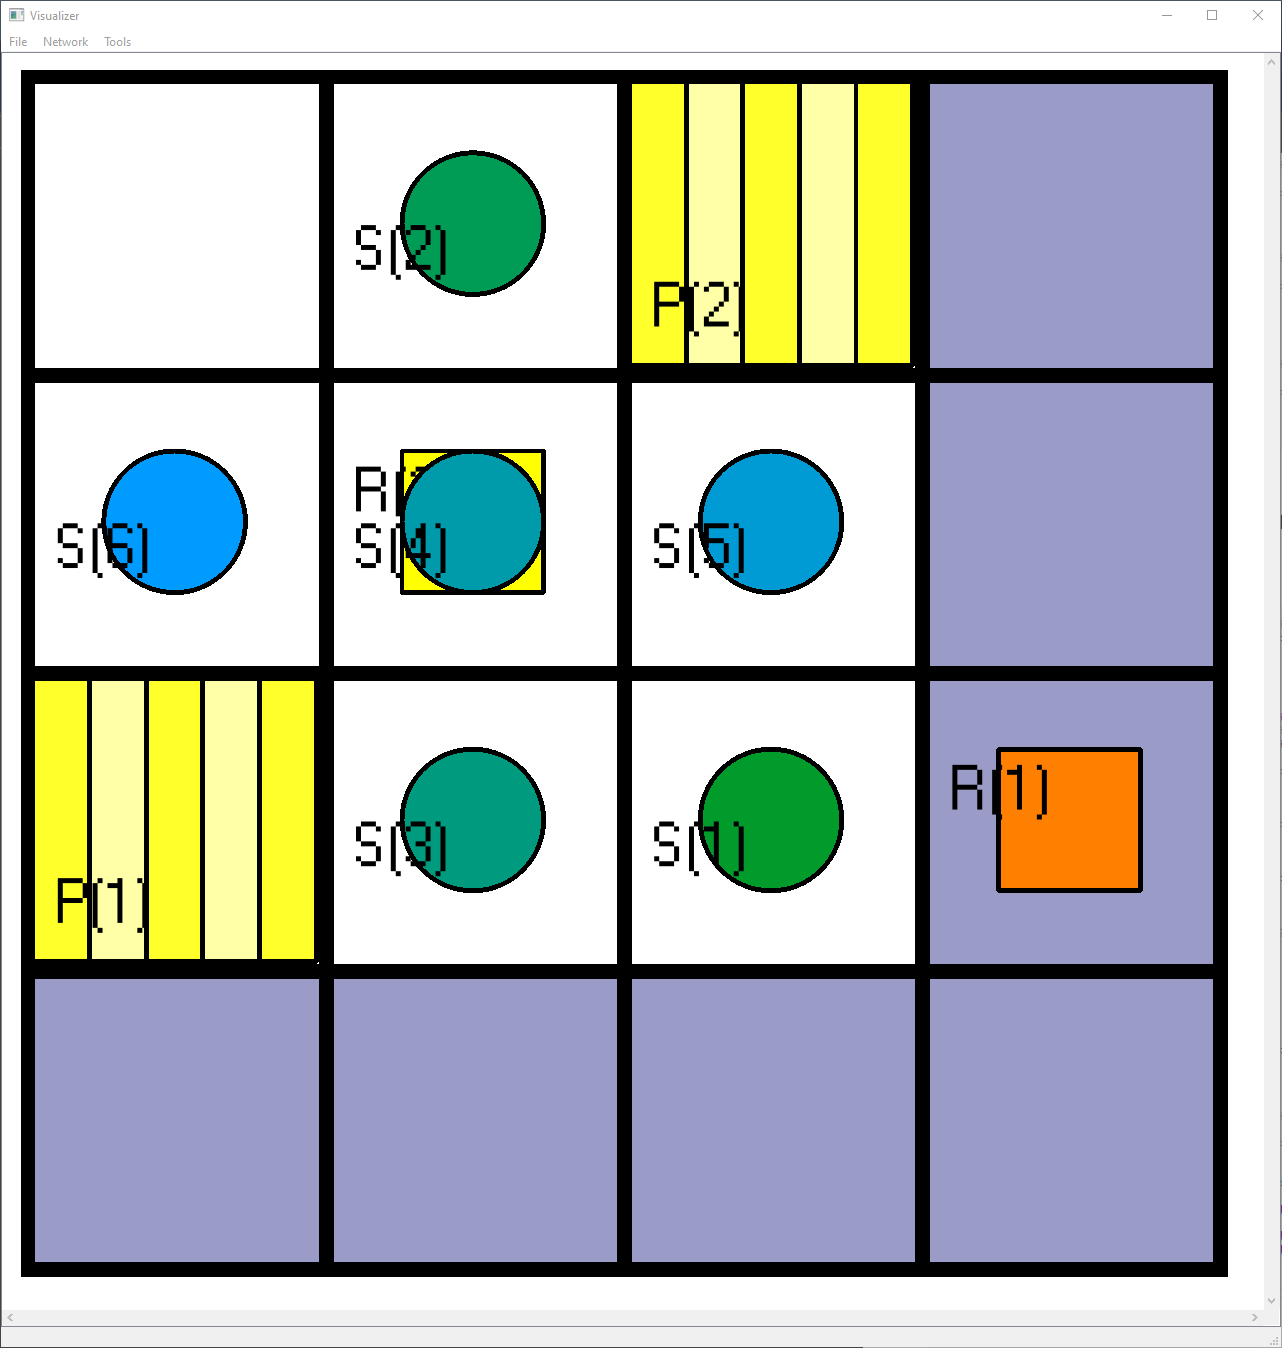
\includegraphics[width=1.3in]{p4_s0.png}}~~%\
  \subfloat[Step 1]{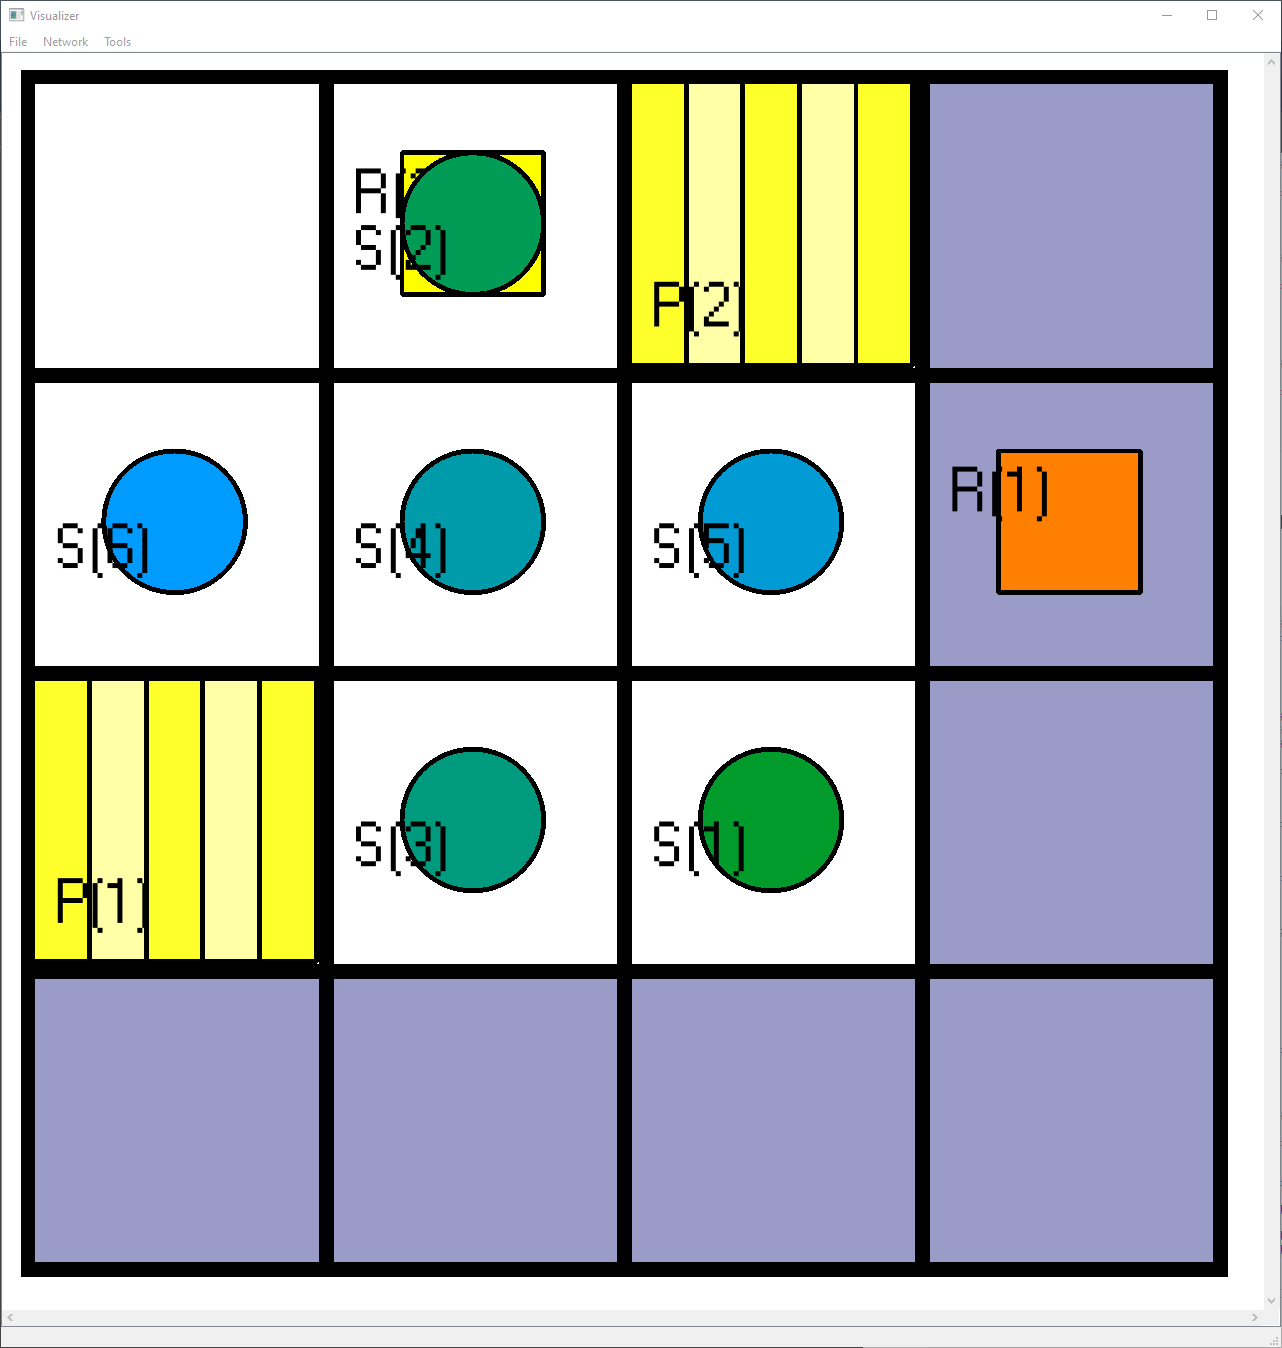
\includegraphics[width=1.3in]{p4_s1.png}}~~%
  \subfloat[Step 2]{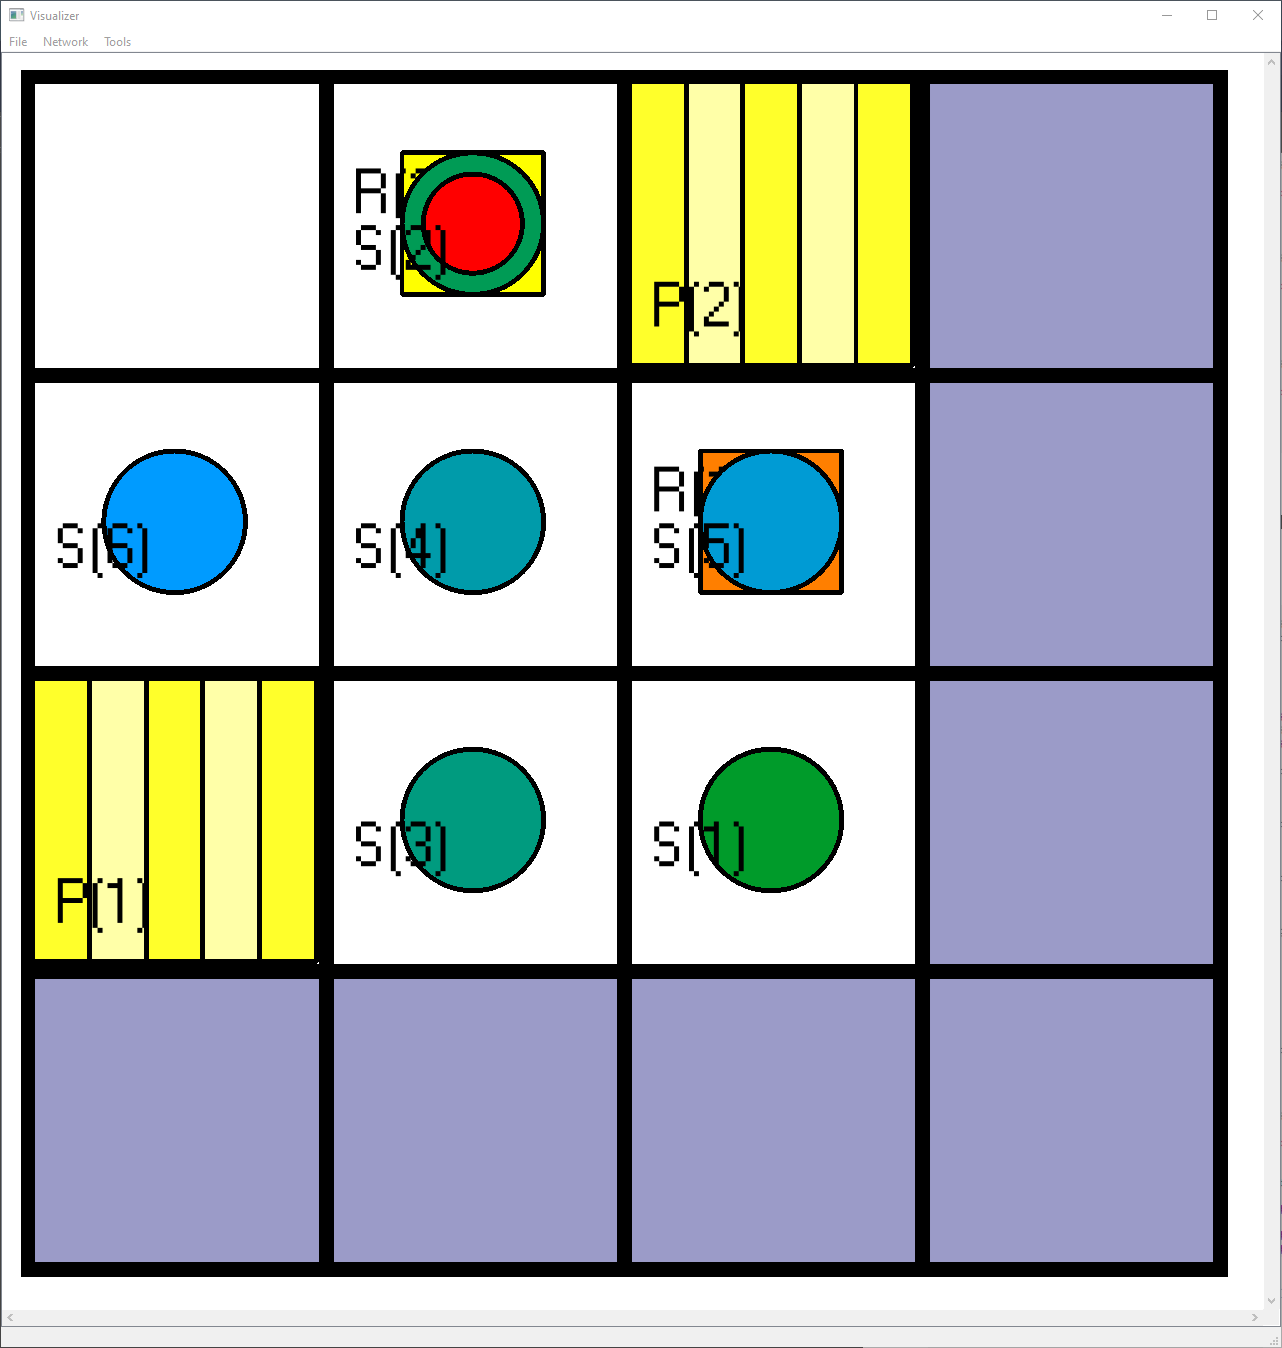
\includegraphics[width=1.3in]{p4_s2.png}}~~%
  \subfloat[Step 3]{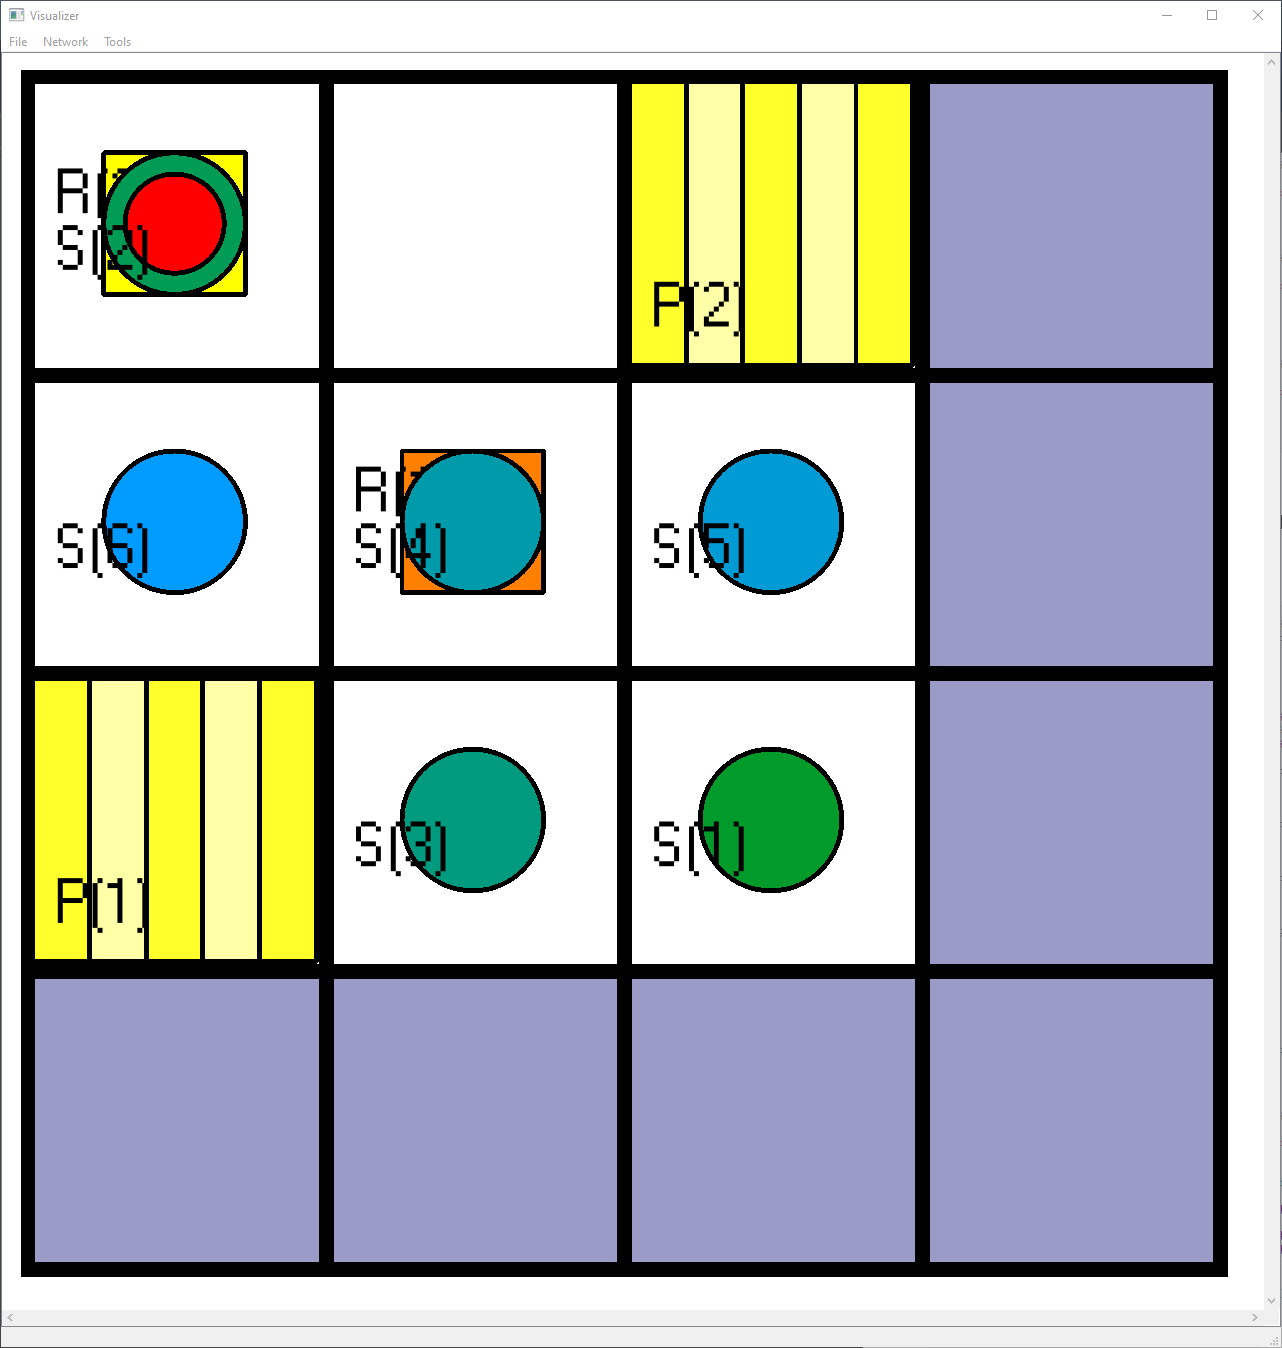
\includegraphics[width=1.3in]{p4_s3.png}}\\%
  \subfloat[Step 4]{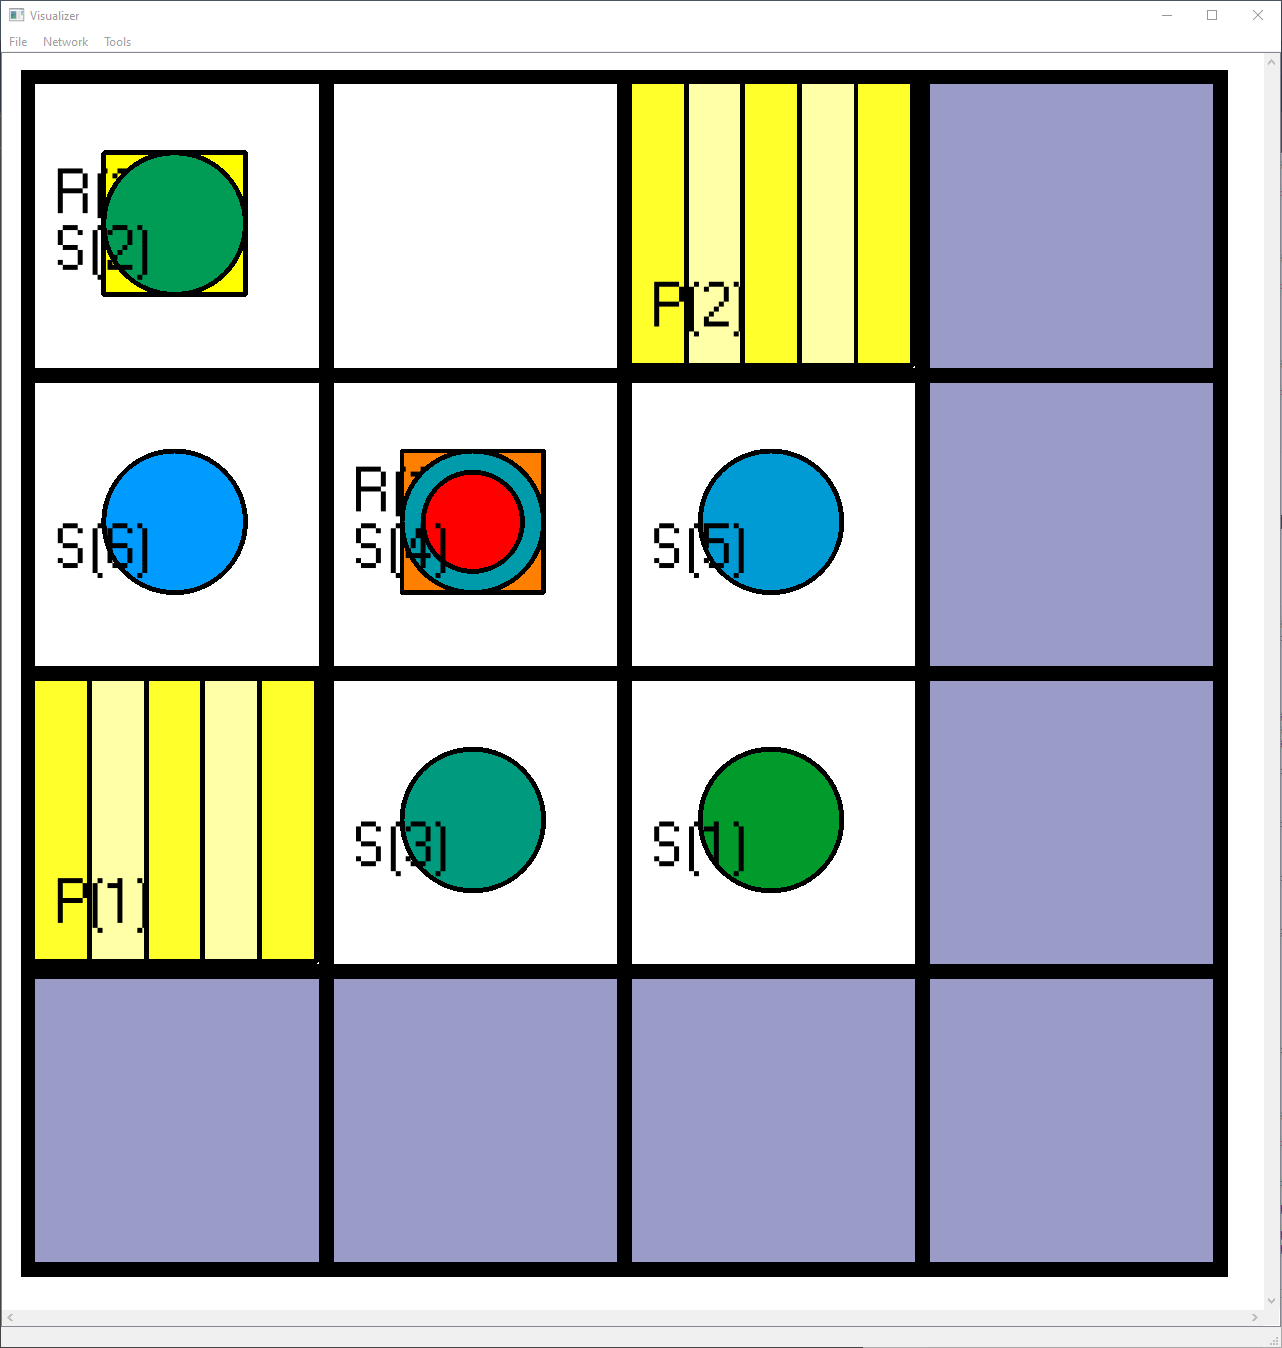
\includegraphics[width=1.3in]{p4_s4.png}}~~%
  \subfloat[Step 5]{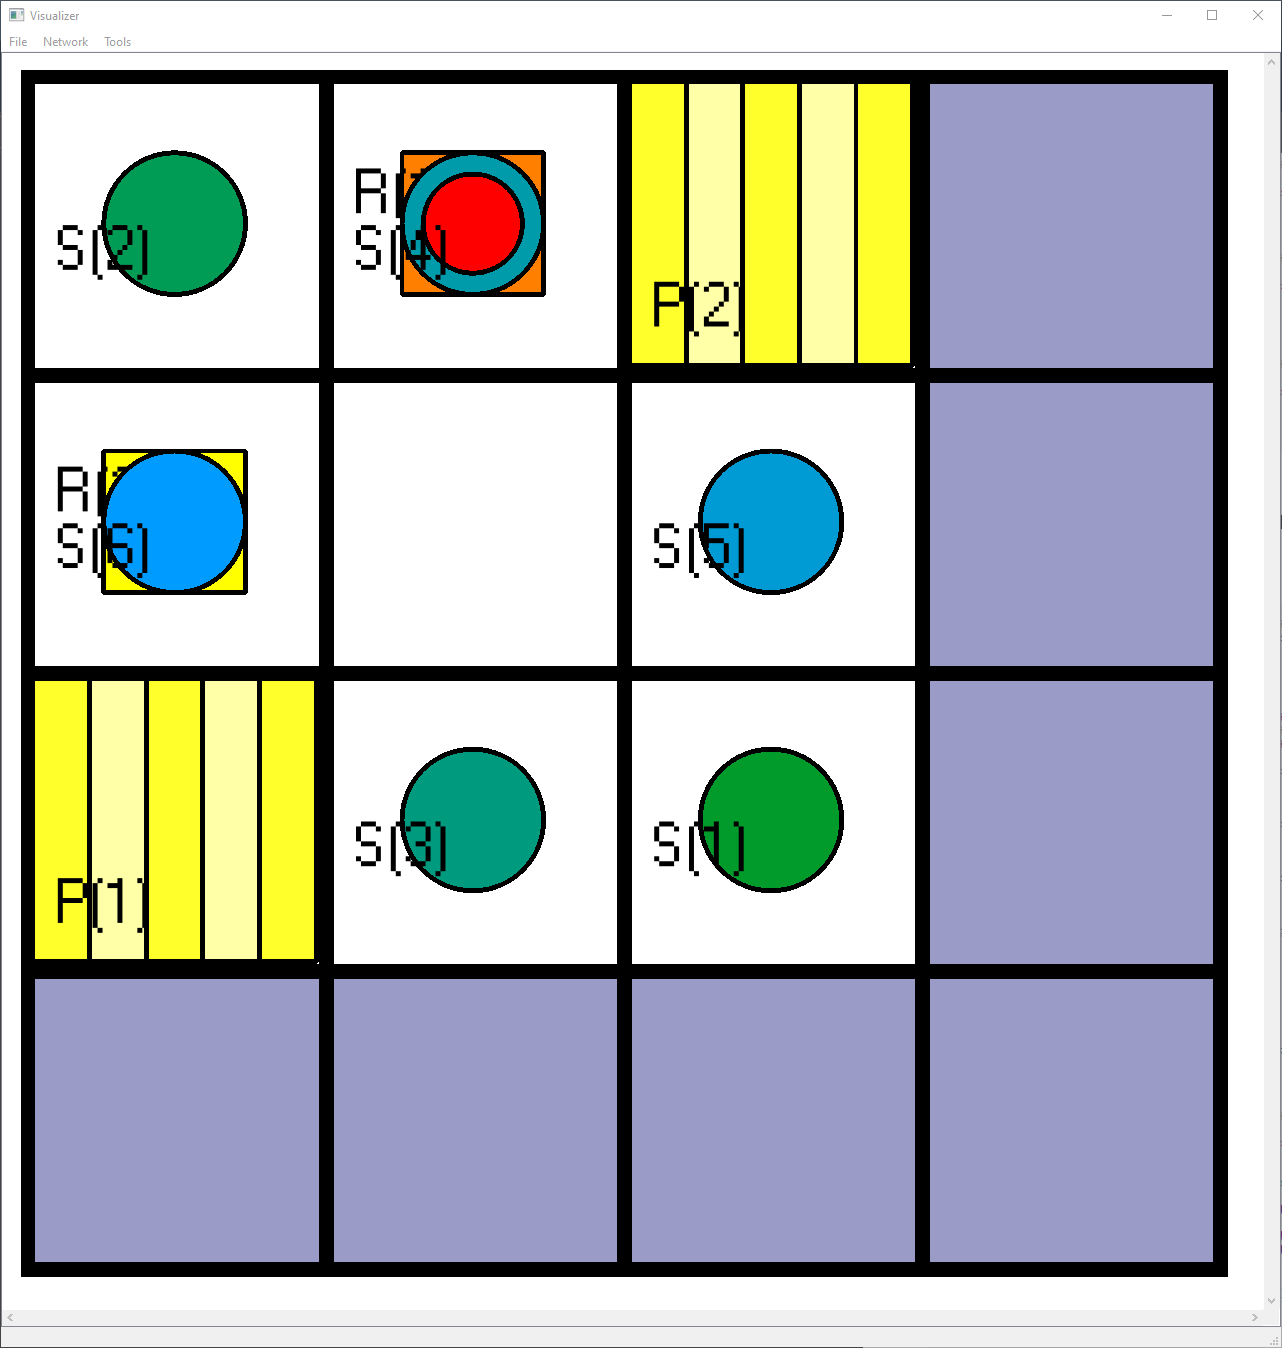
\includegraphics[width=1.3in]{p4_s5.png}}~~%
  \subfloat[Step 6]{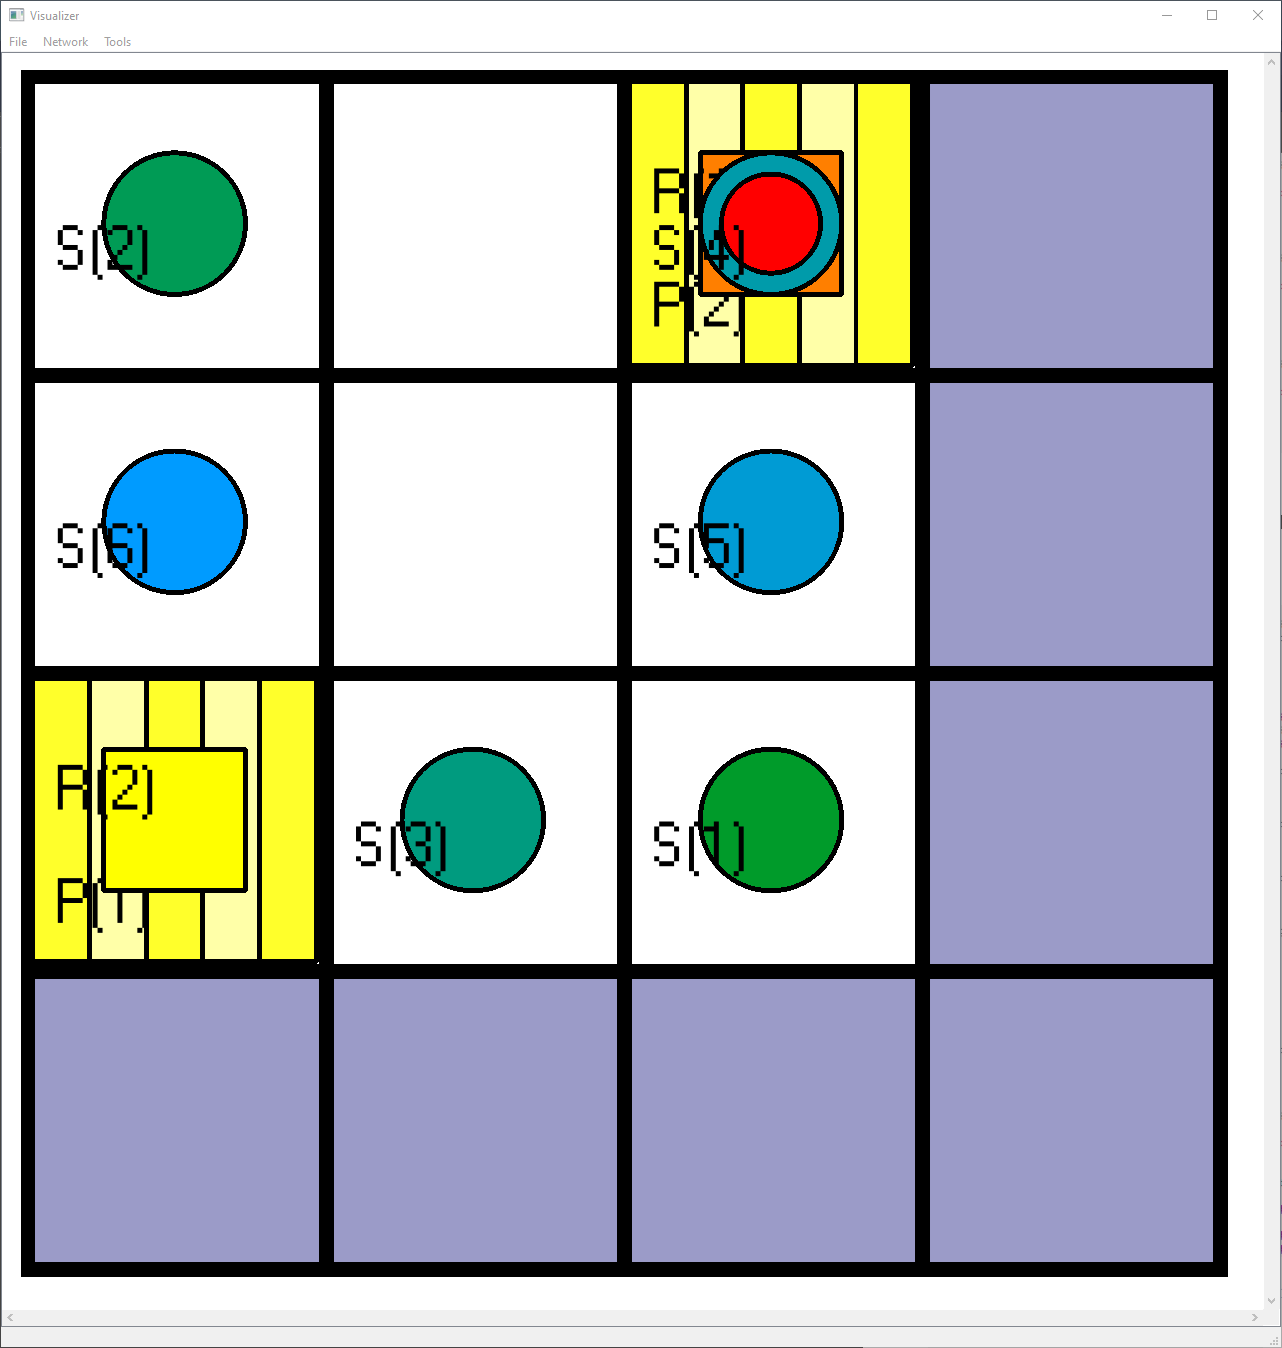
\includegraphics[width=1.3in]{p4_s6.png}}~~%
  \subfloat[Step 7]{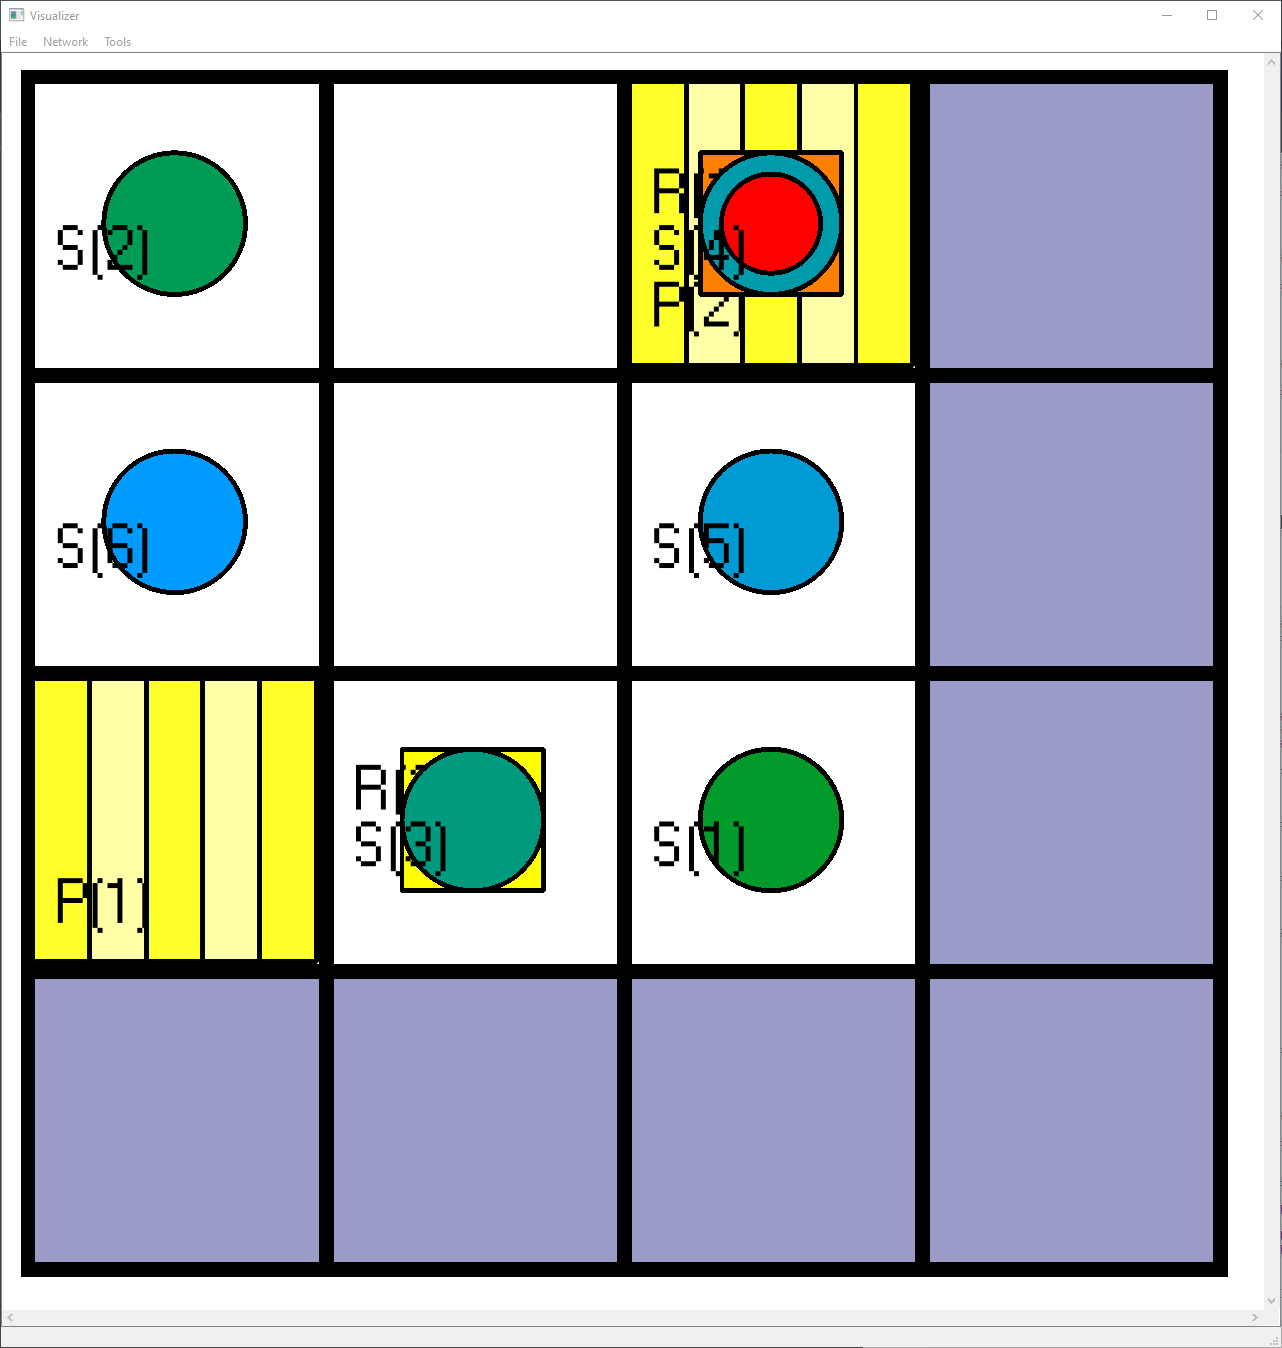
\includegraphics[width=1.3in]{p4_s7.png}}\\%
  \subfloat[Step 8]{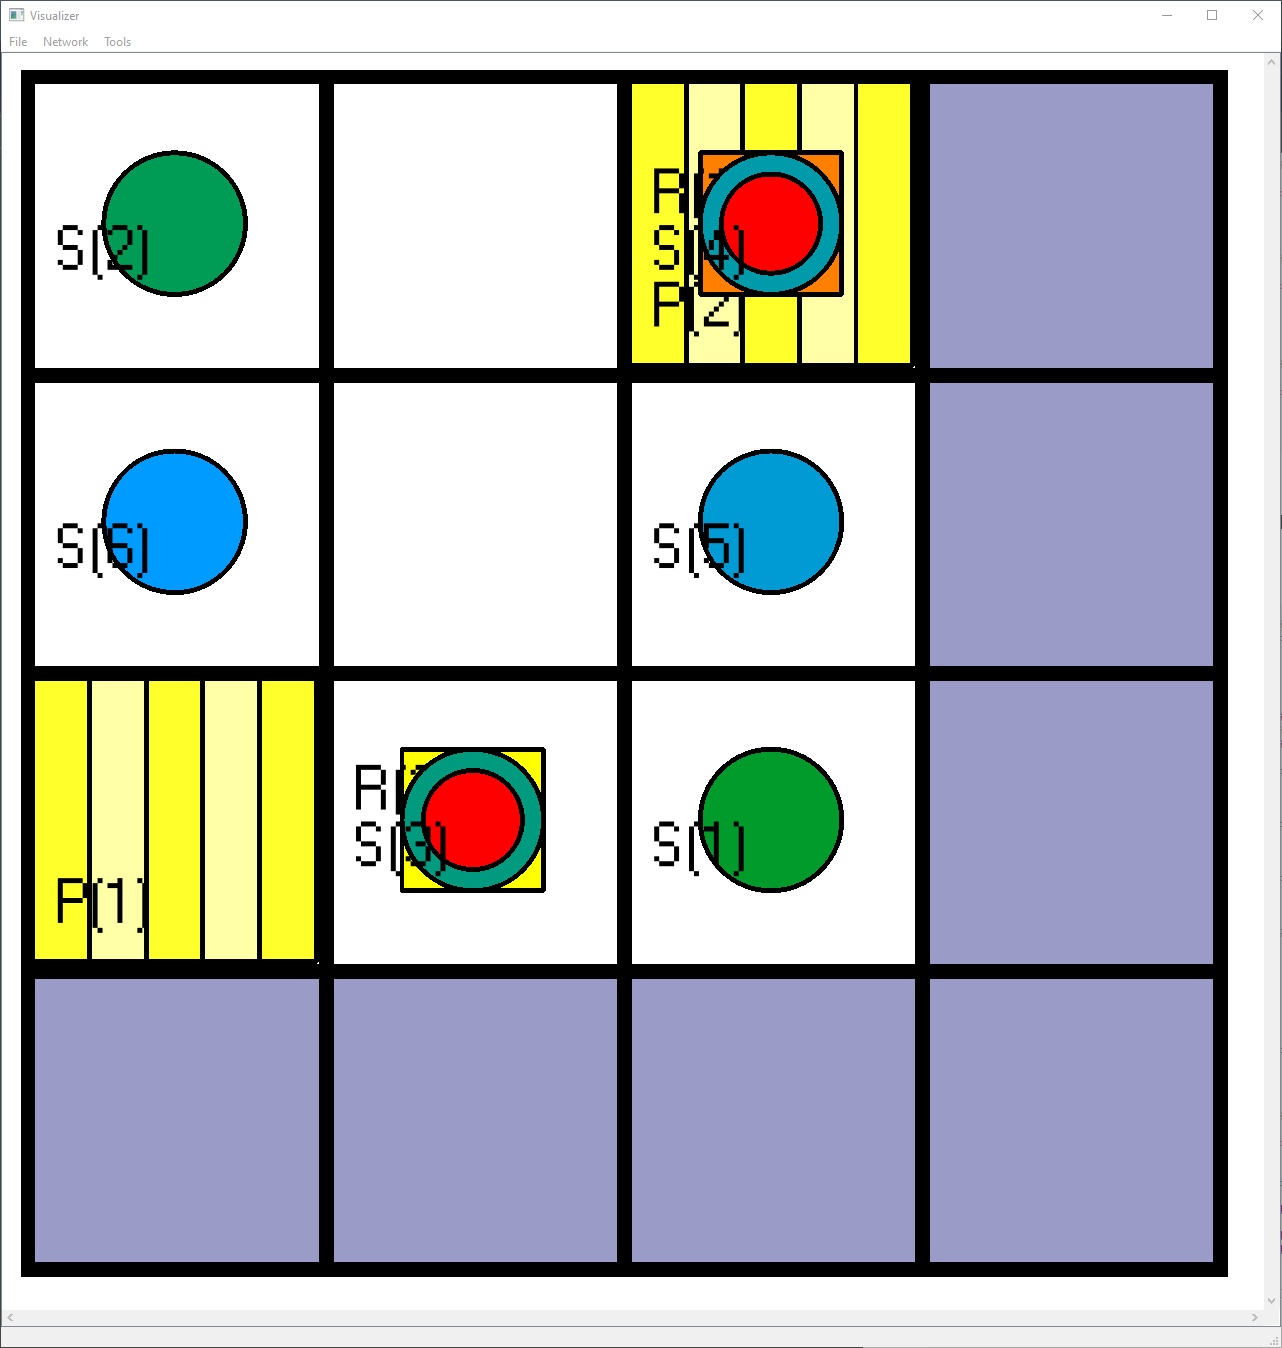
\includegraphics[width=1.3in]{p4_s8.png}}~~%
  \subfloat[Step 9]{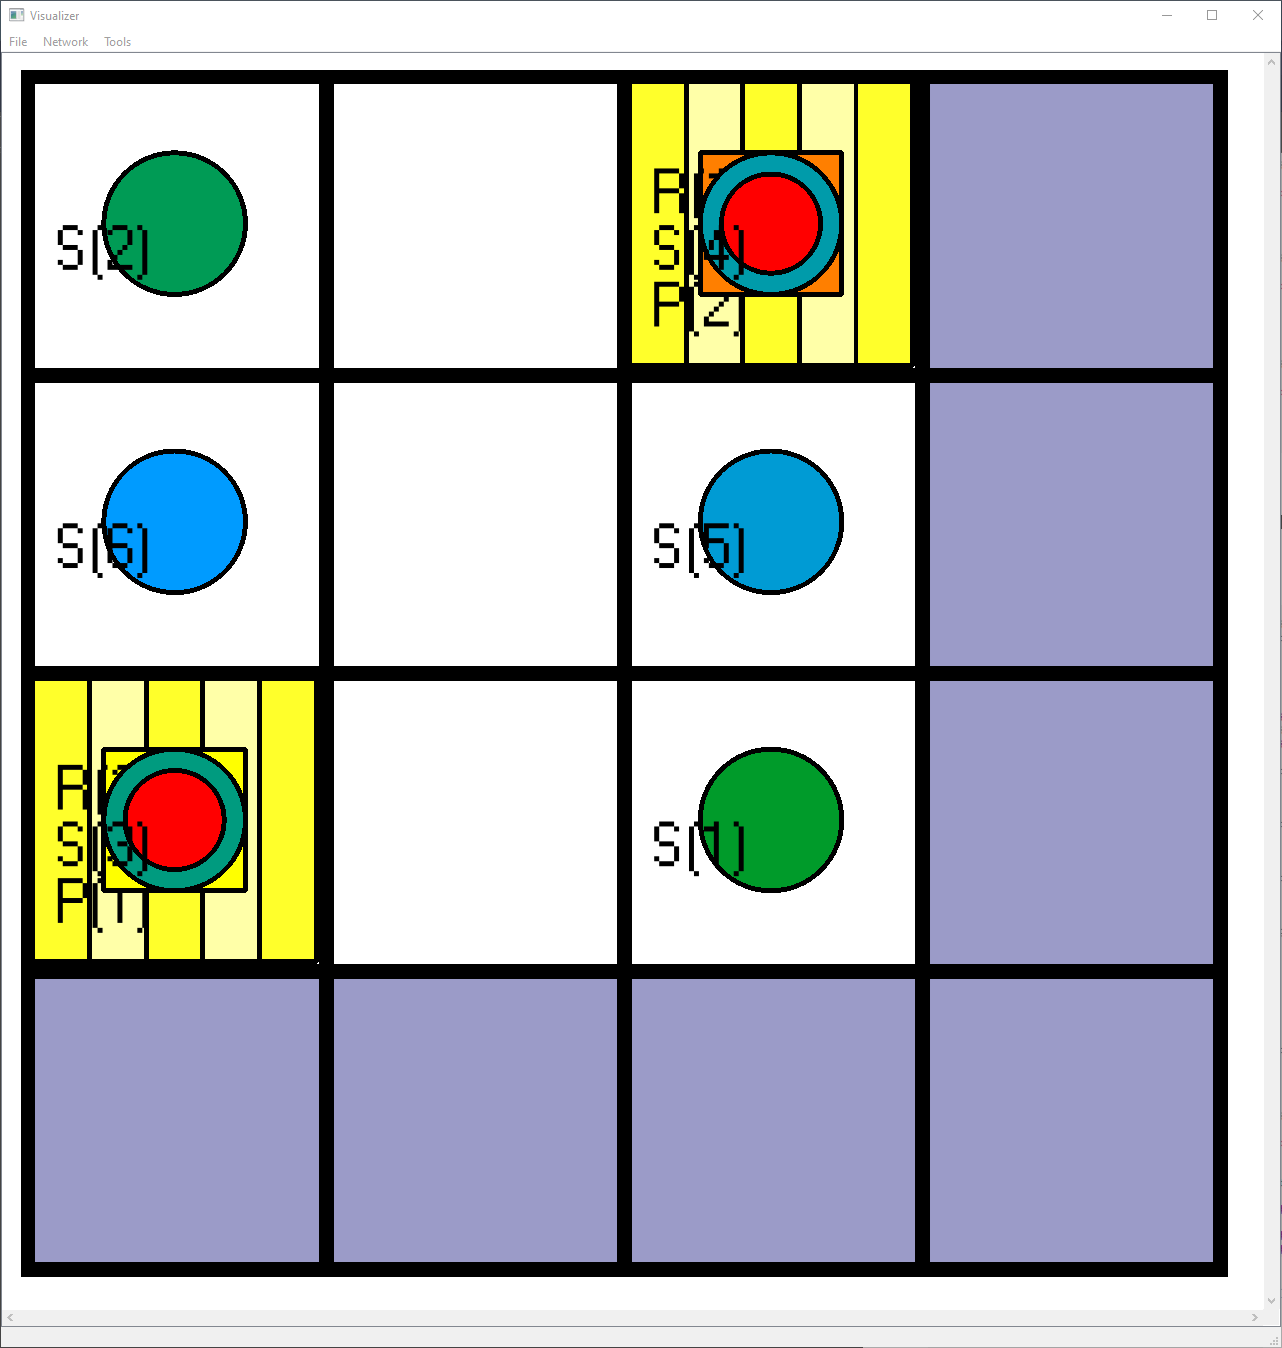
\includegraphics[width=1.3in]{p4_s9.png}}~~%
  \subfloat[Step 10]{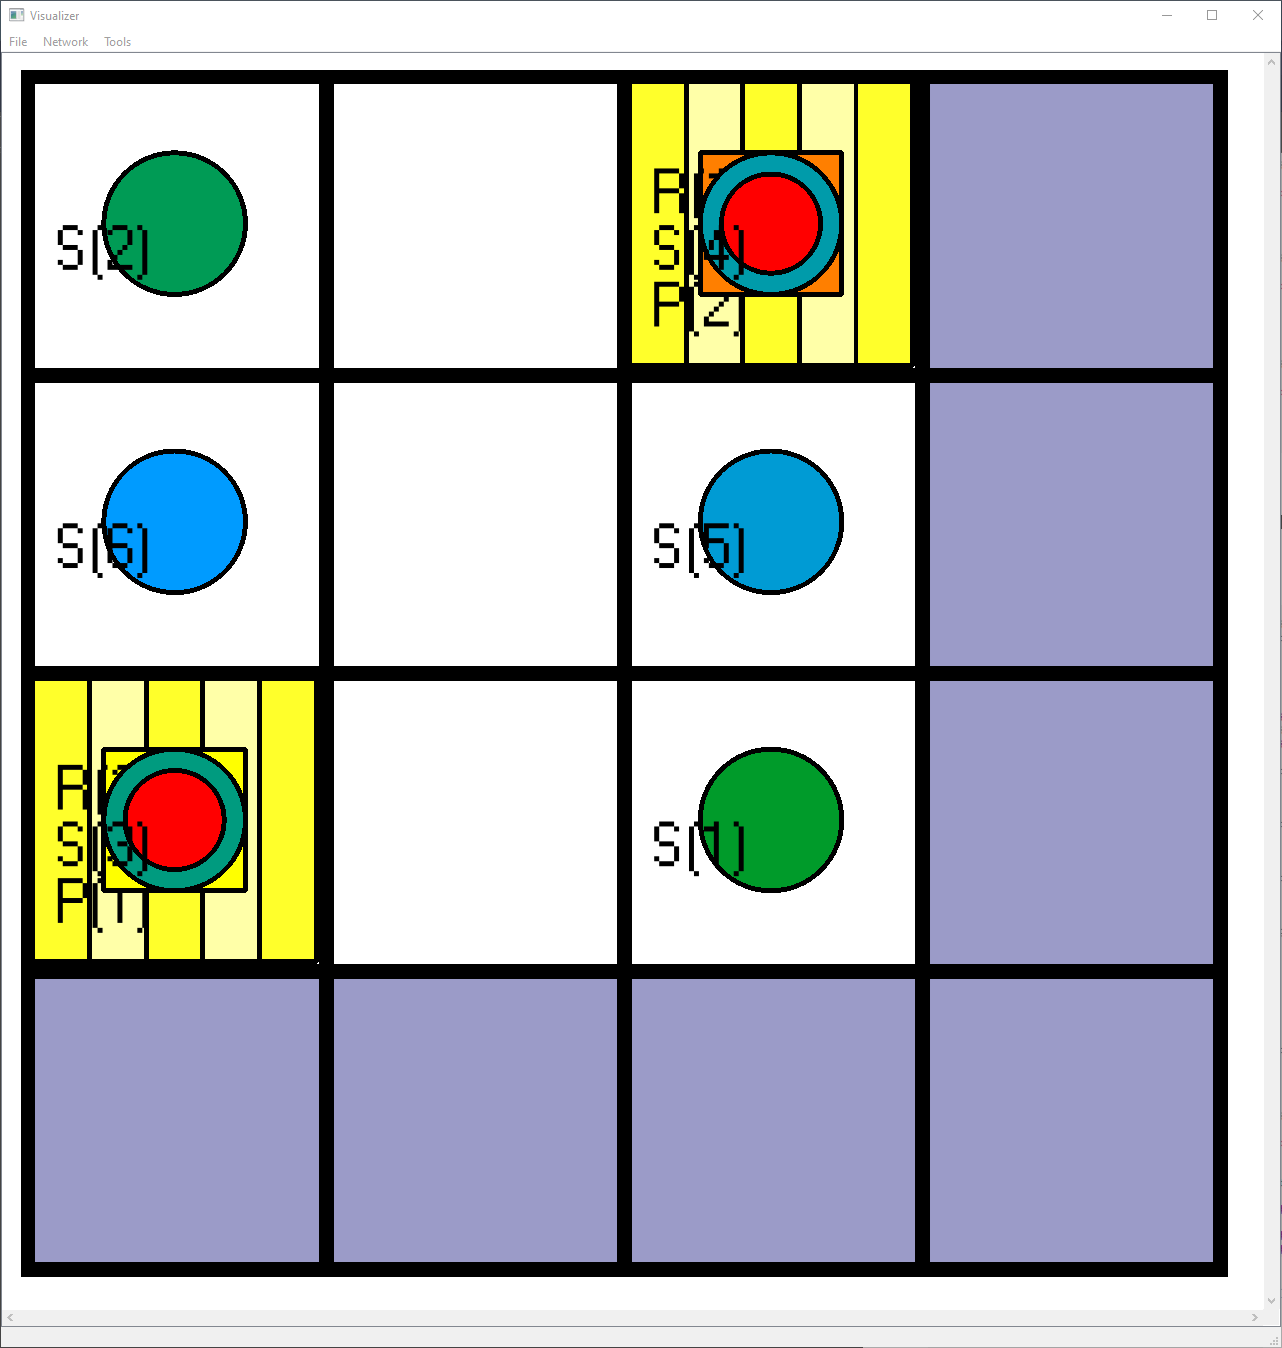
\includegraphics[width=1.3in]{p4_s10.png}}%
  \caption{
    Robot 1 removes a shelf out of the way for Robot 2\\
    Robot 1 is the yellow box and Robot 2 the orange box\\
    Red circle over Robot indicates action of holding the shelf\\
    Step 10 is different from 9 because it includes a Delivery
  }%
  \label{fig:robotRemovesForAnother}%
\end{figure}

\end{document}
